\section{Motivation}
\indent CosmOS is an open-source project that we have initiated since 2020. We aim to create a hybrid operating system that offers performance and safety features within one system.\\
\indent The CosmOS architecture also allows the generation of all configuration code by model descriptions to increase productivity, make code portable, and enforce consistency. We created a set of tools with a graphical user interface to help users with the CosmOS deployment, consisting of configuration, validation, and code generation. \\
\indent It also supports the C/C++ language with the dynamic allocation and allows users to develop more complex algorithms. \\
\indent We developed CosmOS according to safety-critical design principles and coding best practices and we will strive to enhance the overall quality and safety of the software for the future releases.

\section{Architecture}
\indent CosmOS architecture is microkernel-based and implements a near-minimum amount of the operating system’s software.\\ 
\indent The main parts of the CosmOS microkernel is scheduling, memory handling, and data exchange interface. Data exchange interface is the operating system basic inter-program communication model. The microkernel can be easily expanded either with system jobs if it is necessary and make the microkernel modular, even though is highly suggested to implement all services in the user space and use data exchange interface for the inter-program communication as it is shown in the figure \ref{fig:systemArchitecture}.\\
\indent The programs are running in the user space and each of them is encapsulates its threads and tasks, providing them a safe memory space for the data, and heap for the dynamic allocation. This design allows users to implement programs with multiple safety levels without any interference between them. \\
\indent To ensure memory safety, the operating system configuration is completely static that includes also configured programs, tasks and threads and remain constant during the run-time. 
\begin{figure}[H]
\begin{center}
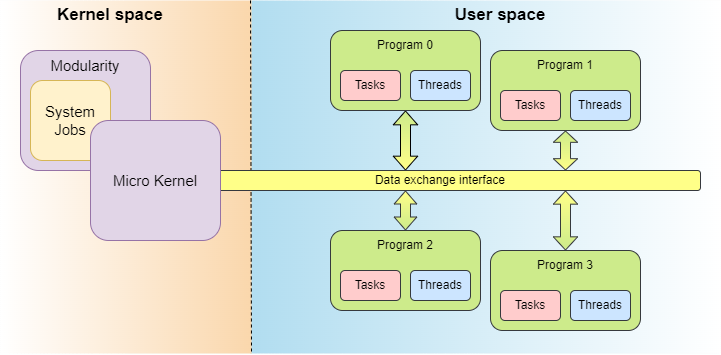
\includegraphics[width=1\textwidth]{images/system_architecture.png}
\caption{System architecture simplified diagram}
\label{fig:systemArchitecture}
\end{center}
\end{figure}

\section{Software layers}
CosmOS is composed of three main software layers:
\begin{itemize}
\vspace{-0.2cm}\item The application layer contains the user code.
\vspace{-0.2cm}\item The core layer contains kernel modules and their configuration without any microcontroller or compiler dependencies. It comprises the configuration (generated) units and non-generated units.
\vspace{-0.2cm}\item The integration layer contains units providing \ac{API} for the core layer, and it is microcontroller-specific.
\end{itemize}


\section{Main features}
We implemented multiple safety concepts to ensure it offers safety and performance features.\\
\indent The following list contains the main features of the CosmOS and CustomBox:
\begin{itemize}
\vspace{-0.2cm}\item The CustomBox \ac{GUI} helps users with configuration, generation and deployment.
\vspace{-0.2cm}\item Support for multi-core microcontrollers.
\vspace{-0.2cm}\item Hybrid scheduling combines the cyclic real-time non-preemptive scheduling and the multi-threading preemptive scheduling.
\vspace{-0.2cm}\item Memory mapping and memory protection of tasks/threads stacks, user program heaps, and user program data.
\vspace{-0.2cm}\item Memory manager supports thread-safe dynamic allocations.
\vspace{-0.2cm}\item Inter-program safe data transfers.
\vspace{-0.2cm}\item Configurable tasks/threads permissions for data transfers.
\vspace{-0.2cm}\item Possibility to implement drivers in application layer with configurable peripheral access.
\vspace{-0.2cm}\item Modular kernel expansion by system jobs with inner scheduling.
\vspace{-0.2cm}\item Configurable synchronization primitives.
\vspace{-0.2cm}\item Highly portable and modular design, which is easy to port and expand.
\end{itemize}


\section{Workflow}
In the figure \ref{fig:systemArchitecture} is shown the workflow diagram of the CosmOS. CustomBox tool helps with most of the configuration steps.\\
\indent First, user has to choose and download the integration and core bundle. These bundles contains all necessary non-generated source code.\\
\indent Later user configures the operating system modules and creates the programs, tasks and threads. After the configuration is completed, user can generate the configuration source code. \\
\indent The last step is to implement user code, compile and flash the board.

\begin{figure}[H]
\begin{center}
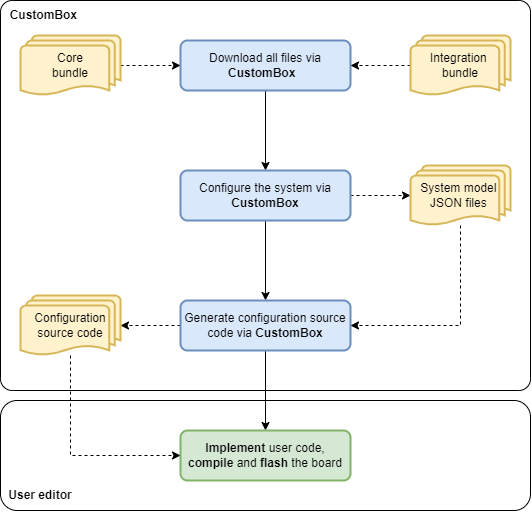
\includegraphics[width=0.9\textwidth]{images/workflow.png}
\caption{CosmOS workflow diagram}
\label{fig:workflow}
\end{center}
\end{figure}

